\chapter{Fugaの設計}
\label{chap:design}
本章では,提案手法を実現するためのソフトウェアシステムとして\textbf{Fuga}\footnote{ふーが.フーガ.}の設計を説明する.
設計および機能の概要を述べたのち,Fugaを構成する各コンポーネントの設計について詳細に説明する.
\section{概要}
Fugaの設計の概要を\figref{fig:system-architecture}に示す.
本システムは,ランサムウェアの侵害を検知し,侵害の影響を受ける直前のデータを退避させることを目的としており,
\textbf{Detector},\textbf{Process Monitor},\textbf{Evacuation Module},\textbf{Data Shelter}の4つのコンポーネントで構成される.
まず,Detectorはランサムウェアの疑いがあるユーザプロセスを特定し,そのプロセスの識別子をProcess Monitorに通知する.
Process MonitorはDetectorから通知を受け取り,指定されたプロセスを監視する.
そして監視対象のプロセスが実行する暗号化関数や関連するシステムコールにフックを挿入する,
このフックにより,暗号化前のファイルコンテンツデータの取得とファイルメタデータの収集が行われる.
取得されたコンテンツデータとメタデータは,Process MonitorによってEvacuation Moduleに送信され,
Evacuation Moduleによって適切な形式に加工された後,
ランサムウェアから隔離されたストレージであるData Shelterに退避される.

% なお,ここでいう「ファイルの侵害」とは,暗号化を行ったりランダムなデータで上書きしたりすることでファイルを利用不可能にする振る舞いを指す.
\begin{figure}[t]
  \centering
  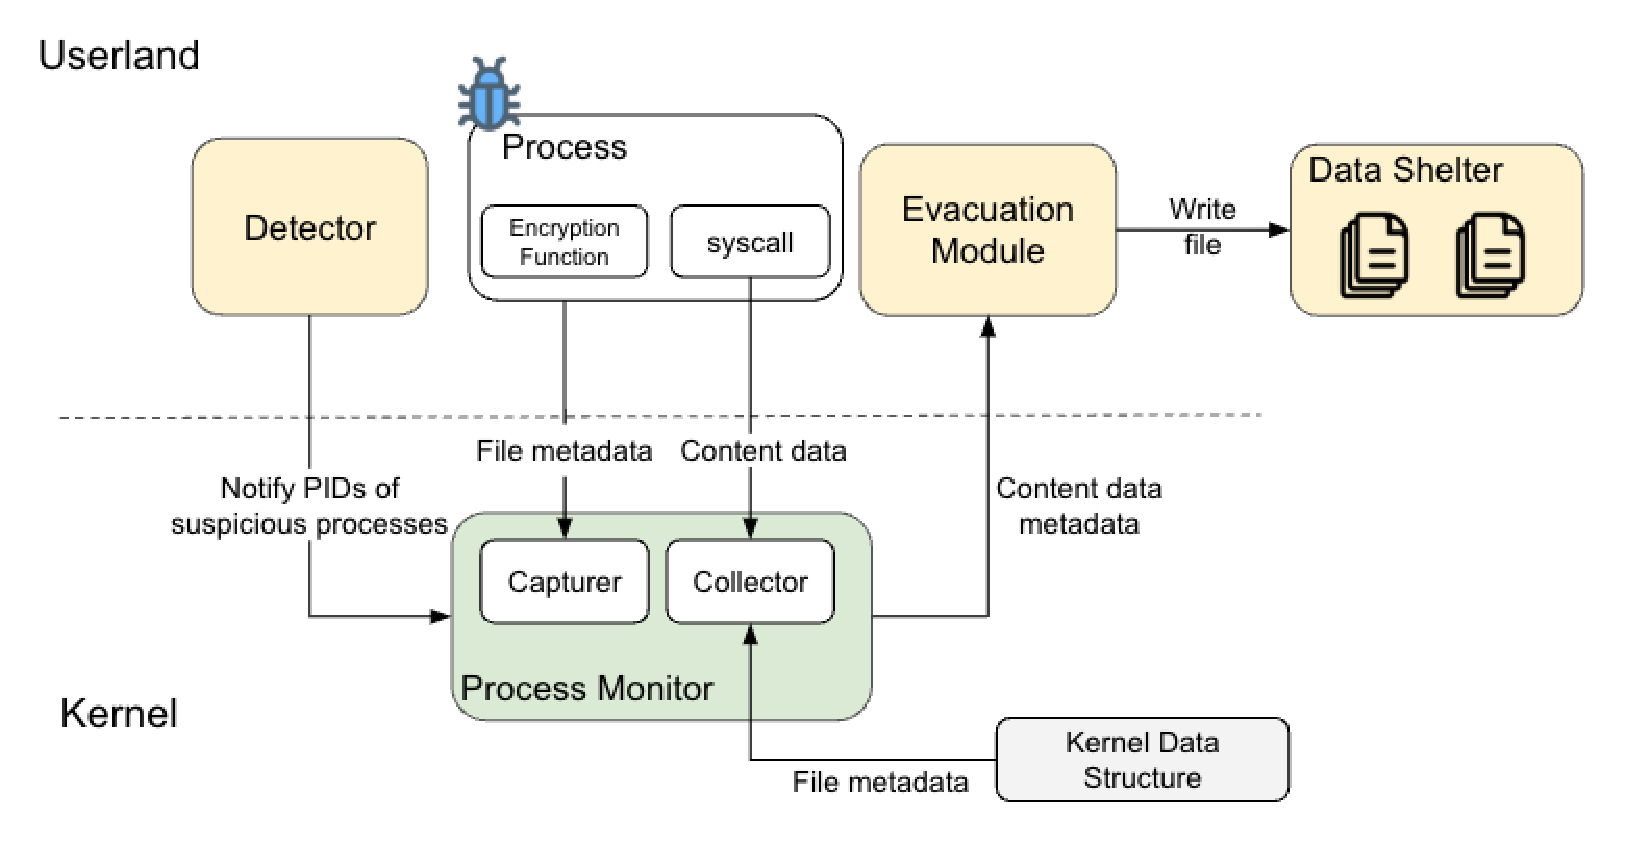
\includegraphics[width=\columnwidth]{doc/img/system_overview.eps}
  \caption{Overview of the design of Fuga.}
  \label{fig:system-architecture}
\end{figure}

\section{各コンポーネントの設計}
% \figref{fig:system-architecture}内の各コンポーネントをそれぞれ説明する.
\subsection{Detector}
Detectorはユーザ空間で実行されるプロセスで,自身以外のユーザプロセスを監視して保守的なランサムウェア検知を行う.
ランサムウェアの可能性が閾値よりも高いプロセスを発見した際に,そのプロセスの識別子をProcess Monitorに通知する.
一度監視対象となったがその後正常なプロセスであると判定された場合も,同様に通知を行う.
なお,\ref{sec:ransom-detect}節で述べたように,ランサムウェアの検知手法は先行研究が多数存在する.
したがって本研究においてDetectorの機能は利用可能であるという前提を置き,その内部実装は本研究のスコープ外とする.

Detectorがランサムウェア検知を保守的に行う方法は採用する検知手法に依存する.
機械学習による検知手法 \cite{alraizza2023ransomware,matos2018rockfs,wan2018feature}では,
機械学習モデルの出力と比較される閾値を小さくすればよい.
悪意スコアを計算する検知手法 \cite{kharraz2017redemption} でも同様である.
ルールベースの検知手法では,ルールセットの一部を無視することで保守的な検知を行うことができる.

Detectorをユーザ空間で実行されるプログラムとして設計した理由は,既存のランサムウェア検知手法の利用を容易にするためである.
単純なルールベースの検知手法であれば,カーネル空間のプログラムとして実装することも可能であるが,
機械学習を用いた手法などは,カーネル空間での実装は不可能ではないにせよ技術的に困難である.

\subsection{Process Monitor}
Process Monitorはカーネル空間で実行されるプログラムであり,Detectorが指定したユーザプロセスを監視している.
Process Monitorは,暗号化前の平文データを取得する\textbf{Capturer}モジュールと,
ファイルのメタデータを収集する\textbf{Collector}モジュールで構成される.
Capturerが取得した平文データとCollectorが収集したメタデータは,
一つのデータ構造に格納されてEvacuation Moduleに送信される.

Capturerは監視対象のプロセスが実行する暗号化関数をフックし,関数の引数に渡される平文データのポインタをキャプチャする.
その後ポインタが指すバッファのデータを対象のユーザプロセスのメモリ空間からカーネルメモリ空間へとコピーすることで平文データを取得する.

CollectorはCapturerと連携し,ファイルの復旧に必要なメタデータ,具体的にはファイルパスと
コンテンツデータのオフセットを以下のように収集する.
\\
ファイルパスの取得:ファイルを開くシステムコールをフックし,ファイルの相対パスをシステムコールの引数から取得する.
さらに,カーネル内構造体にアクセスして対象プロセスの現在の作業ディレクトリ(Current Working Directory: CWD)を取得する.
システムコールにはファイルの絶対パスが引数として渡されることがあるが,この場合はCWDの取得は不要となる.
% 相対パスとCWDから,操作対象のファイルの絶対パスを構成する.
\\
オフセットの取得:
あるファイルが監視対象プロセスによって開かれたら,
そのファイルのオフセットを管理する変数を初期化する.
ファイルのコンテンツデータをメモリ上に読み込むシステムコール,
およびファイルの現在のオフセットを操作するシステムコールをフックし,
各ファイルのオフセットの変化量を取得する.この値を用いてファイルのオフセットを管理する変数を動的に更新する.

Process Monitorをカーネル空間で実行されるプログラムとして設計した理由は,
ユーザ空間でのプロセス間のデータコピーが技術的およびセキュリティ上の制約により困難であるためである.
共有メモリや明示的なプロセス間通信を利用すればデータの受け渡しは可能だが,ランサムウェアのプロセスが
Process Monitorとそのような通信プロトコルを形成することはありえない.
また,カーネル空間で動作するプログラムを利用したランサムウェア対策には,ランサムウェアによって無効化される可能性が極めて低いという利点がある\cite{mitigation-modern}.
権限昇格を行う高度なランサムウェアがProcess Monitorを無効化する可能性は残るものの,Process Monitorの無効化はランサムウェアの活動として検知されやすいため,
攻撃者にとってリスクが高いといえる.

% Process Monitorをカーネル空間で実行されるプログラムとして設計した理由は,
% あるユーザプロセスから別のユーザプロセスへのデータコピーを実現することが非常に困難なためである.
% 共有メモリや明示的なプロセス間通信を利用すればデータの受け渡しは可能であるが,
% Fugaにおいて監視されるユーザプロセスがそのような合意をProcess Monitorと形成することはできない.
% 加えて,カーネル空間のプログラムを用いたランサムウェア対策は,ランサムウェアによって無効化される可能性が非常に低い \cite{mitigation-modern}という利点がある.
% 権限昇格を行うランサムウェアにはProcess Monitorを無効化する可能性もあるが,
% Process Monitorの無効化はランサムウェアの特徴であるため,検知される可能性が高い.

\subsection{Evacuation Module}
Evacuation Moduleはユーザ空間で実行されるコンポーネントである.
このコンポーネントはまず,Process Monitorからコンテンツデータおよびメタデータを受け取る.
この際,Process MonitorとEvacuation Moduleとの間でデータの表現形式が異なる場合は,必要に応じてデータ形式を適切に変換する.
そしてこれらのデータを用いて,侵害されるファイルのデータを退避する処理を実行する.
具体的な処理の内容は,Data Shelterの形態によって決定される.処理の概要を\figref{fig:how-to-evacuate}に示す.
詳細は後述するが,Data Shelterの形態としてはローカルストレージ,NAS (Network Attached Storage),またはリモートホストなどが考えられる.
\begin{figure}[t]
  \centering
  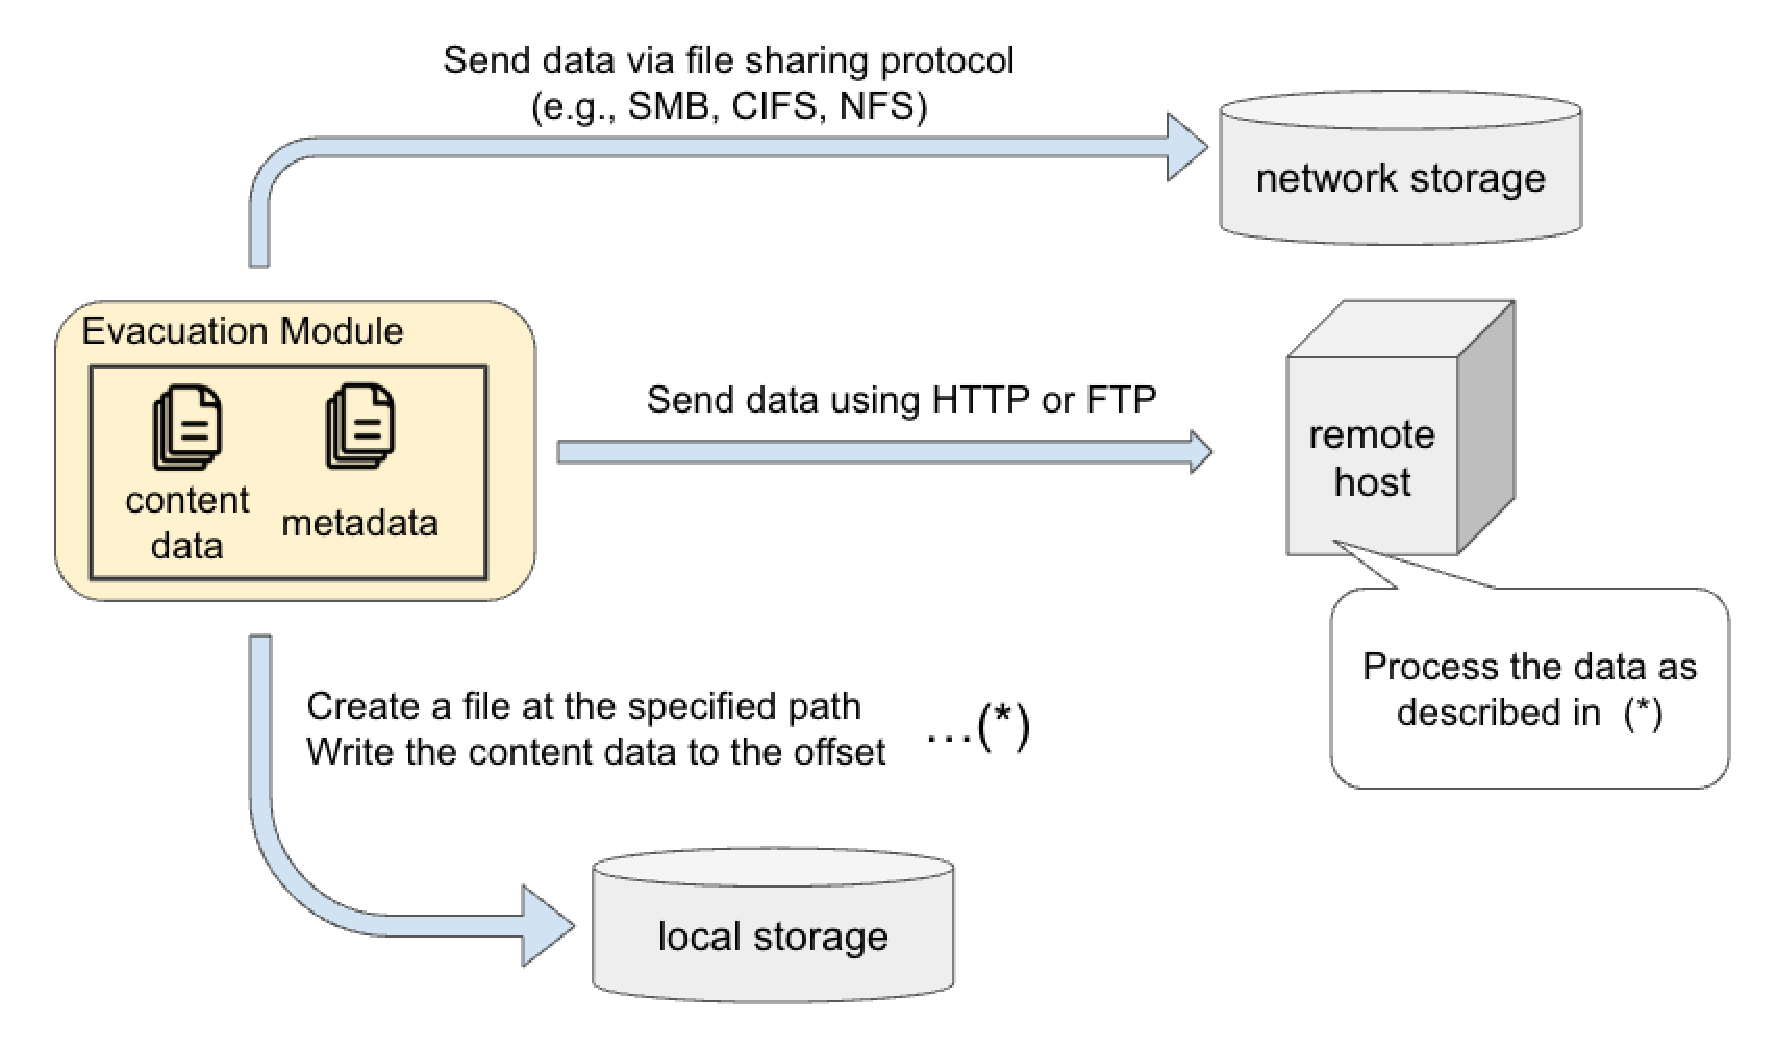
\includegraphics[width=0.9\columnwidth]{doc/img/how-to-evacuate.eps}
  \caption{The Evacuation Module processes and transfers content data and metadata to a Data Shelter,
    which may be a local storage, network storage, or remote host, depending on its configuration.}
  \label{fig:how-to-evacuate}
\end{figure}


Evacuation Moduleは,その実装がData Shelterの形態に依存することを考慮し,ユーザ空間で実行されるプログラムとして設計されている.
この設計により,実装やデバッグ,修正がカーネル空間プログラムよりも容易に行える.
また,Data Shelterの新しい形態への対応も簡便化される.
たとえば,リモートホストをData Shelterとして使用する場合,既存のAPIやライブラリを利用することで,
新しい通信プロトコル(e.g., HTTP,FTP)へのサポートを迅速かつ省力的に追加できる.
同様に,ローカルストレージをData Shelterとして使用する場合も,複数のファイルシステムを柔軟にサポートできる.
一方で,Evacuation Moduleをカーネル空間プログラムとして設計することも可能ではあるが,
% その場合ユーザ空間とカーネル空間との間のコンテキストスイッチの削減により性能が向上する可能性がある.
カーネルプログラミングは,システムクラッシュやセキュリティ脆弱性のリスクが高く,バグの影響が深刻になる可能性がある.
そのため,ユーザ空間での設計は,開発の安全性や柔軟性を確保しながら,必要な機能拡張に対応しやすい選択肢である.

\subsection{Data Shelter}
\label{subsec:data-shelter}
ランサムウェアによる侵害から隔離されたデータ領域を,本稿ではData Shelterと呼ぶ.
Fugaの利用者は,ランサムウェア攻撃が発覚した後,Data Shelterに退避されたファイルを取得し,
侵害されたファイルを復旧することができる.

\figref{fig:how-to-evacuate}に示すように,Data Shelterはローカルストレージ,NAS,またはリモートホストなどの形態で構成可能である.
特に,リモートホストをData Shelterとして利用する場合,Evacuation Module側でファイルを作成して転送する方法と,
Evacuation Moduleが送信したデータを元にData Shelter側でファイルを作成する方法のいずれかを選択することができる.
\figref{fig:how-to-evacuate}では後者の処理を示している.
後者の場合,Data Shelterとなるリモートホスト上でスナップショットを作成したり,
ファイル保存時にシャーディング \cite{what-is-sharding}やその他の冗長性向上手法を適用したりすることで,
データバックアップをさらに堅牢にすることができる.
% Data Shelterとして使用するデータストアにはいくつか選択肢が考えられる.
% アクセス制限を適用したローカルのディレクトリが最もシンプルであるが,
% NASなどを利用して,Fugaを展開するホストの外部にData Shelterを配置してもよい.
